\documentclass[a4paper, 12pt]{article}
\usepackage[a4paper, total={6in, 8in}]{geometry}
\geometry{
	a4paper,
	left = 1.5 cm,
	right = 1.5 cm,
	top = 2cm,
	bottom = 2.5 cm,
}
\usepackage[T1]{fontenc}
\usepackage{pythontex}
\usepackage{hhline}
\usepackage{array,booktabs}
\newcolumntype{M}[1]{>{\centering\arraybackslash}m{#1}}
\usepackage[table]{xcolor}
\usepackage{caption}
\usepackage{makecell}
\usepackage{lipsum}
\usepackage{pifont}
\usepackage{amssymb}
\usepackage{amsmath}
\usepackage[utf8]{inputenc}
\usepackage[italian]{babel}
\usepackage{graphicx}
\graphicspath{ {./images/} }
\usepackage{spverbatim}
\usepackage{float}
\usepackage{url}
\usepackage{xstring}
\usepackage{hyperref}
\usepackage{xcolor}
\usepackage{upquote}
\definecolor{linkcolor}{RGB}{1,1,87}
\hypersetup{
    colorlinks,
    citecolor=black,
    filecolor=black,
    linkcolor=linkcolor,
    urlcolor=blue
}
\usepackage{fancyvrb,newverbs,xcolor}
\definecolor{cverbbg}{gray}{0.93}
\definecolor{cellcolor}{RGB}{165,194, 242}
\usepackage{xifthen}
\usepackage{multirow}
\usepackage{adjustbox}
\usepackage{listings}
\lstset{
  basicstyle=\ttfamily,
  backgroundcolor=\color{cverbbg},
  breaklines=true,
  frame=lines,
  framerule=1pt,
  numbers=left,
  numbersep=10pt, 
  keywordstyle=\color{blue},
  commentstyle=\color{green!60!black},
  stringstyle=\color{red},
  showstringspaces=false,  
  framextopmargin=1.5ex,
  framexbottommargin=1.5ex,
  framexleftmargin={\dimexpr 1.5em+3pt},
  xleftmargin={\dimexpr 1.5em+3pt},
  linewidth={\dimexpr \linewidth-3pt}
}

% following restart section enumeration in different \part
\usepackage{chngcntr}
\counterwithin*{section}{part}

\newcommand{\makesub}[1]{%
  \saveexpandmode\noexpandarg
  \StrSubstitute{#1}{\_}{_}[\temp]%
  \restoreexpandmode%
}

\newcommand{\target}[1]{%
  \makesub{#1}%
  \hypertarget{\temp}{}%
}

\newcommand{\attach}[1]{%
  \makesub{#1}%
  \hyperlink{\temp}{\emph{#1}}%
}
\newcommand{\attachcode}[1]{%
  \makesub{#1}%
  \hyperlink{\temp}{\code{#1}}%
}

\newcommand{\code}[1]{\colorbox{cverbbg}{	exttt{\detokenize{#1}}}}
%\newcommand{\code}[1]{\colorbox{cverbbg}{\texttt{\StrSubstitute{#1}{_}{\_}}}}

\newcommand{\linux}{\textit{Linux}}
\newcommand{\win}{\textit{Windows}}
\newcommand{\nota}[1]{\textbf{Nota}: #1}
\newcommand{\memo}[1]{\textbf{Memo}: #1}
\newcommand{\esempio}[1]{\textbf{Esempio}: #1}
\newcommand{\tbs}{\textbackslash}
\newcommand{\Null}{\code{NULL}}
\newcommand{\api}{\emph{API}}
\newcommand{\key}[1]{\texttt{\StrSubstitute{#1}{_}{\_}}}
\usepackage{eurosym}

\newcommand{\paramtable}[2][]{%
\ifthenelse{\isempty{#2}} {\input{|"/home/luca/latex_scripts/generate_param_table.py '#1'"}} {\input{|"/home/luca/Scrivania/MA/homeworks/homework-04/report/scripts/generate_param_table.py '#1' '#2'"}}%
}

\newcommand{\hr}[0]{\begin{center}%
\line(1,0){450}%
\end{center}%
}

\newcommand{\xmark}[0]{\ding{55}}
\newcommand{\vmark}[0]{$\checkmark$}

\newenvironment{myverb}
 {\SaveVerbatim{cverb}}
 {\endSaveVerbatim
  \flushleft\fboxrule=0pt\fboxsep=.5em
  \colorbox{cverbbg}{%
    \makebox[\dimexpr\linewidth-2\fboxsep][l]{\BUseVerbatim{cverb}}%
  }
  \endflushleft
}

\setcounter{tocdepth}{4}
\setcounter{secnumdepth}{4}
\setlength\parindent{0pt}
\newcommand{\image}[1]{\input{|"/home/luca/latex_scripts/add_image.py '#1'"}}

%%%%%%%%%%%%%%%%%%%%%
\newcommand{\bup}[0]{$\mathcal{B} \cup \mathcal{P}$}


\begin{document}

\title{
    \textbf{    
        \emph{Simulazione PMCSN}
    }
}
\author{Luca Mastrobattista, 0292461}
\date{} %no date wanted
\maketitle  



\tableofcontents

\newpage
\section{Traccia della Simulazione}
\subsection{Caso di studio}
Si vuole valutare l'idea di aprire un locale in un piccolo paese. L'attività dovrà offrire ai clienti servizi di bar e di pizzeria. Il locale è già provvisto di tutto l'arredamento e lo si affitterà per un costo 1500 $\mbox{\euro}$ al mese. Il pizzaiolo scelto per i servizi di pizzeria ha comunicato che, nel forno presente, si possono preparare contemporaneamente al massimo 2 pizze, ognuna delle quali può essere preparata con un tempo medio di 3 minuti. Inoltre, si è già trovato un accordo con lui: lavorerà ogni giorno della settimana dalle ore 19:00 alle ore 23:00, percependo una paga di 50 $\mbox{\euro}$ al giorno con il vincolo che tutte le ordinazioni arrivate prececedentemente alle 23:00 
verranno sempre completate, anche se per farlo dovrà continuare a sfornare pizze oltre questo orario. Per quanto riguarda le richieste al bar, si vuole che "l'ultimo giro" venga chiamato alle ore 03:00, senza accettare altre richieste successive a quell'orario ma completando tutte quelle ancora presenti. \newline
Dopo un'osservazione settimanale di altri locali che offrono servizi simili, si è notato che il numero di clienti che arrivano al locale si differenzia per fasce orarie della giornata diverse. Inoltre, nel fine settimana, la frequenza delle richieste nelle fasce orarie identificate è maggiore rispetto a quella settimanale. Infine, si è osservato che nella fascia oraria tra le 15:00 e le 18:00 le richieste sono talmente poche che non è conveninente mantenere il locale aperto. Si riportano di seguito delle tabelle riassuntive per le frequenze di arrivo:

\target{tabelle riassuntiva dei tassi di arrivo}
\begin{table}[!htb]
\begin{minipage}{.5\linewidth}
\centering
    
\begin{tabular}{ |c|c|c| }
\hline
\cellcolor{cellcolor}Fascia oraria & \cellcolor{cellcolor}$\lambda${\textsubscript{B,W}} & \cellcolor{cellcolor}$\lambda${\textsubscript{P,W}} \\
	\hline
	\hline
    07:00 $\rightarrow$ 11:00 & 30 j/h & \xmark \\
    \hline
    11:00 $\rightarrow$ 15:00 & 12.5 j/h & \xmark \\
    \hline
    15:00 $\rightarrow$ 18:00 & \xmark & \xmark \\
    \hline
    18:00 $\rightarrow$ 19:00 & 25 j/h & \xmark \\
    \hline
    19:00 $\rightarrow$ 23:00 & 12.5 j/h & 10 j/h \\
    \hline
    23:00 $\rightarrow$ 02:00 & 10 j/h & \xmark \\
    \hline
    \end{tabular}
	\bigskip 
	       
	\textit{Frequenze di arrivo settimanali} 
\end{minipage}
\begin{minipage}{.5\linewidth}
\centering
\begin{tabular}{ |c|c|c| }
\hline
\cellcolor{cellcolor}Fascia oraria & \cellcolor{cellcolor} $\lambda${\textsubscript{B,WE}} & \cellcolor{cellcolor}$\lambda${\textsubscript{P,WE}} \\
	\hline
	\hline
	07:00 $\rightarrow$ 13:00 & 30 j/h & \xmark \\
	\hline
	13:00 $\rightarrow$ 18:00 & 20 j/h & \xmark \\
    \hline
	15:00 $\rightarrow$ 18:00 & \xmark & \xmark \\
    \hline
    18:00 $\rightarrow$ 19:00 & 45 j/h & \xmark \\
    \hline
    19:00 $\rightarrow$ 23:00 & 22.5 j/h & 40 j/h \\
    \hline
    23:00 $\rightarrow$ 03:00 & 20 j/h & \xmark \\
    \hline
    \end{tabular}
	\bigskip 
	   
	\textit{Frequenze di arrivo fine-settimanali} 
\end{minipage} 
\end{table}

\bigskip

\subsection{Obiettivi}
Obiettivo dell'analisi è la valutazione del numero di baristi da
assumere, col fine ultimo di massimizzare i guadagni. Si considera una paga di 40 $\mbox{\euro}$ al giorno per ognuno di loro, assumendo per loro turni di 8 ore. Si assume che ogni barista sia in grado di servire un'ordinazione in 2 minuti, durante i quali si dedica esclusivamente a quella richiesta. Si assume inoltre che il prezzo medio delle richieste di tipo B sia di 5 $\mbox{\euro}$, mentre quello delle richieste di tipo P sia di 7 $\mbox{\euro}$. Si vuole, però, che i seguenti vincoli siano sempre rispettati:
\begin{itemize}
  \item Ogni ordinazione al bar deve essere servita in un tempo strettamente minore di 3 minuti;
  \item Ogni ordinazione per la pizzeria sia servita in un tempo strettamente minore di 10 minuti 
\end{itemize}

\newpage
\section{Modello concettuale}
\subsection{Visualizzazione grafica}
	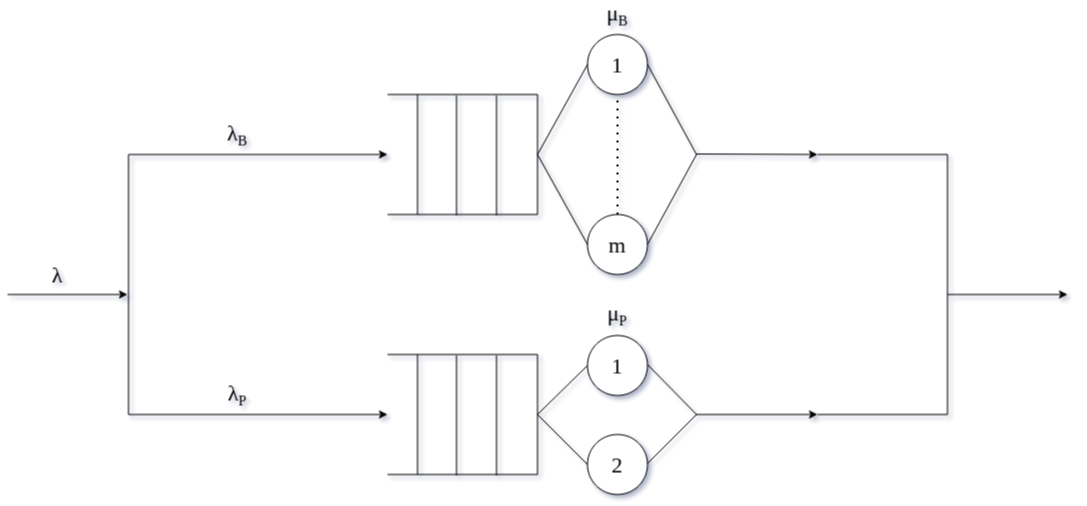
\includegraphics[width=\textwidth]{conceptual_model}
La frequenza di arrivo $\lambda$ si compone della frequenza di arrivo
$\lambda\textsubscript{B}$ e $\lambda\textsubscript{P}$, che sono rispettivamente i tassi di arrivo per richieste al bar e alla pizzeria. Una opportuna coda per ogni tipologia rappresenta la lista di attesa della tipologia stessa. Ogni servente di tipo \emph{B} rappresenta un barista assunto, che lavora con una frequenza $\mu\textsubscript{B}$. Ogni servente di tipo \emph{P}, invece, rappresenta una delle due richieste che il pizzaiolo è in grado di gestire contemporaneamente.


\subsection{Eventi del sistema e variabili di stato}
\subsection{Eventi}
\begin{center}
\begin{tabular}{ |c|c|c|c| }
	\hline
    \cellcolor{cellcolor}Indice & \cellcolor{cellcolor}Descrizione & \cellcolor{cellcolor}Attributo 1 & \cellcolor{cellcolor}Attributo 2 \\
    \hline
    \hline
    0 & Arrivo di tipo B & t & x \\
    \hline
    1 & Completamento dal server $B_1$ & t & x \\
    \hline
    .. & .. & t & x \\
    \hline
    m & Completamento dal server $B_m$ & t & x \\
    \hline
    m + 1 & Arrivo di tipo P & t & x \\
    \hline
    m + 2 & Completamento dal server $P_1$ & t & x \\
    \hline
    m + 3 & Completamento dal server $P_2$ & t & x \\
    \hline
    m + 4 & Evento di campionamento & t & x \\
    \hline
\end{tabular}
\end{center}
L'attributo \emph{t} indentifica il tempo schedulato per la successiva occorrenza
dell'evento di quel tipo; l'attributo \emph{x} identifica lo stato di attività
dell'evento.

\subsection{Variabili di stato}
\begin{itemize}
  \item $l\textsubscript{B}(t)$: numero di richieste di tipo B al centro all'istante $t$
  \item $l\textsubscript{P}(t)$: numero di richieste di tipo P al centro all'istante $t$
  \item $X\textsubscript{s}(t)$: stato del servente $s$ all'istante $t$, 
  con $s \in$ \bup, dove \bup{} è l'insieme dei serventi di tipo \textit{B} unito all'insieme dei serventi di tipo \textit{P}.
  \[
      X\textsubscript{s}(t) = 
  \begin{cases}
      1& \text{se servente s è occupato}\\ 
      0              & \text{altrimenti}
  \end{cases}
  \]	
\end{itemize}

\section{Modello delle specifiche}

\subsection{Periodo di osservazione}
Il periodo di osservazione è quello di un intero anno e ogni giorno si osserva l'intera giornata lavorativa costituita dalle due fasce orarie riportate precedentemente nelle \attach{tabelle riassuntiva dei tassi di arrivo}.

\subsection{Distribuzione degli arrivi}
I valori dei vari tassi di arrivo sono stati raccolti analizzando un caso reale, anche se si tratta comunque di una stima. Per rappresentare il processo degli arrivi è stata utilizzata la distribuzione esponenziale, utilizzando $\lambda$ diversi per ogni fascia oraria. Inoltre, all'interno della singola fascia oraria, gli arrivi potrebbero essere modellati come una distribuzione gaussiana, centrata attorno all'ora in cui le richieste sono più probabili. A partire da questa osservazione, si è scelto di utilizzare la distribuzione esponenziale per modellare gli arrivi, ma la media utilizzata è pesata opportunamente per una probabilità che è tanto più alta quanto più il tempo di simulazione è vicino all'ora di massima affluenza per quella fascia oraria. Per modellare questo, si definiscono delle frequenze di interarrivo medie per ogni fascia oraria, riportate qui in minuti:
\bigskip

\begin{minipage}{.5\textwidth}
\centering             
\begin{tabular}{ |c|c|c| }
	\hline
    \cellcolor{cellcolor} Fascia oraria & \cellcolor{cellcolor}$\lambda${\textsubscript{B,W}} & \cellcolor{cellcolor}$\lambda${\textsubscript{P,W}} \\
	\hline
    \hline

	07:00 $\rightarrow$ 11:00 & 0.5 j/min & \xmark \\

    \hline
    

	11:00 $\rightarrow$ 15:00 & 0.21 j/min & \xmark \\

    \hline
    

	18:00 $\rightarrow$ 19:00 & 0.42 j/min & \xmark \\

    \hline
    

	19:00 $\rightarrow$ 23:00 & 0.21 j/min & 0.17 j/min \\

    \hline
    

	23:00 $\rightarrow$ 02:00 & 0.17 j/min & \xmark \\

    \hline
\end{tabular}
\bigskip
              
\textit{Frequenze di arrivo settimanali}
\end{minipage}
%
\begin{minipage}{.5\textwidth}
\centering
\begin{tabular}{ |c|c|c| }
	\hline
    \cellcolor{cellcolor}Fascia oraria & \cellcolor{cellcolor}$\lambda${\textsubscript{B,WE}}
    &\cellcolor{cellcolor} $\lambda${\textsubscript{P,WE}} \\
    \hline
    \hline
    

	07:00 $\rightarrow$ 11:00 & 0.5 j/min & \xmark \\ 

    \hline
    

	11:00 $\rightarrow$ 15:00 & 0.34 j/min & \xmark \\

    \hline
    

	18:00 $\rightarrow$ 19:00 & 0.75 j/min & \xmark \\

    \hline
    

	19:00 $\rightarrow$ 23:00 & 0.375 j/min & 1 j/min \\

    \hline
    

	23:00 $\rightarrow$ 02:00 & 0.34 j/min & \xmark \\

    \hline
\end{tabular}
\bigskip
              
\textit{Frequenze di arrivo fine-settimanali} 
\end{minipage} 
\bigskip

Per ogni fascia oraria si definisce una distribuzione di probabilità gaussiana:\\

\begin{table}[H]
\centering
\begin{tabular}{ |c|c|c| }
	\hline
    \cellcolor{cellcolor} Fascia oraria & \cellcolor{cellcolor}$\mu$ & \cellcolor{cellcolor}$\sigma$\\
	\hline
    \hline

  	07:00 $\rightarrow$ 11:00 & 8 & 1.2 \\
    \hline	
	
	11:00 $\rightarrow$ 15:00 & 13.5 & 2 \\
    \hline
  
	18:00 $\rightarrow$ 19:00 & 18.5 & 0.4 \\  
    \hline
    
	19:00 $\rightarrow$ 23:00 & 22.5 & 2\\
    \hline
    
    23:00 $\rightarrow$ 02:00 & 24 & 0.9 \\
    \hline    
\end{tabular}
\end{table}

La loro rappresentazione grafica è riportata \hyperlink{rappresentazione grafica gaussiane}{in fondo al documento}. 
\bigskip

Ora, supponiamo di essere all'istante di simulazione $t_0$ di un giorno settimanale, nella prima fascia oraria; in questo caso $\lambda = 0.5\ j/min$ .  Per generare il prossimo tempo di interarrivo, si definisce:
\[
\lambda' = \lambda \cdot f^n(t_0)
\]
dove $f^n(t_0)$ è il valore della distribuzione normale relativa alla fascia oraria valutata in $t_0$ e normalizzata rispetto alla fascia oraria. Nell'esempio:
\[
f^n(t_0) = \frac{f(t_0)}{F(11) - F(7)}
\]
con $F(x)$ funzione cumulativa della distribuzione gaussiana relativa alla fascia oraria 07:00 $\rightarrow$ 11:00.\\
Dopo aver calcolato in questo modo $\lambda'$, si procede a generare il nuovo tempo di interarrivo con \texttt{Exponential(1/}$\lambda'$\texttt{)}.\\

Non si è usata una gaussiana direttamente come distribuizione del tempo di interarrivo perché avrebbe modellato una cosa diversa: avrei rappresentato che i tempi sono molto più vicini al valor medio della distribuzione all'interno dell'intero intervallo, invece si vuole modellare che il tempo di interarrivo diminuisce in un intorno di un tempo specifico




\subsection{Assunzioni}
\begin{itemize}
  \item Stato iniziale vuoto: 
  \[ 
    l\textsubscript{B}(0) + l\textsubscript{P}(0) = P(0) + B(0) = 0 
\]
  Come conseguenza, il primo evento deve essere necessariamente un arrivo e, in particolare, è un arrivo di tipo \textit{B}: la pizzeria apre alle 19.
  \item Stato finale di ogni giorno vuoto:
\[
    X\textsubscript{s}(T) = 0\ \ \ \forall s \in \mathcal{B} \cup \mathcal{P}
\]
  Con $T$ tempo di chiusura giornaliero e $\mathcal{B} \cup \mathcal{P}$ l'unione dell'insieme dei serventi di tipo \textit{B} e \textit{P}. Come conseguenza, l'ultimo evento non può essere un arrivo, e sarà quindi o una partenza o un campionamento.

  \item I tempi di servizio di ognuno dei serventi si assumono  esponenziali e indipendenti dalla fascia oraria. In particolare, ogni servente di tipo \textit{B} lavora con frequenza media pari a $\mu\textsubscript{B} = \frac{1}{2}\ j/min$; ogni servente di tipo \textit{P} lavora con frequenza media pari a $\mu\textsubscript{P} = \frac{1}{3}\ j/min$.

  
\end{itemize}

\newpage
\section{Modello computazionale}
Il modello computazionale è stato sviluppato in \emph{Python} ed è il programma \key{simulation.py}; i parametri configurabili sono definiti invece nel file \key{configurations.py}.  

\subsection{configurations.py}
File di configurazione che definisce le costanti per:
\begin{itemize}
  \item Slot temporali in cui vengono cambiate le frequenze di interarrivo
  \item La durata di ogni slot temporale
  \item Tempi in cui si attivano e disattivano gli eventi di arrivo
  \item La durata della simulazione
  \item Numero di serventi di tipo B e P
  \item Tempi di arrivo per i due tipi 
  \item Frequenze di interarrivo, per ogni tipo e per ogni fascia oraria, sia
per i giorni infra-settimanali che fine-settimanali
  \item La paga media per ogni servente di tipo B e di tipo P
  \item Il costo medio di ogni richiesta di tipo B e di tipo P
  \item Il costo mensile per l'affitto del locale
  \item Il tasso dell'iva
  \item Il costo medio mensile delle bollette 
\end{itemize}

\subsection{simulation.py}
\begin{itemize}
  \item \emph{indexes}: array che memorizza [$B(t)$, $P(t)$]
  \item \emph{numbers}: array che memorizza [$l\textsubscript{B}(t)$,
$l\textsubscript{P}(t)$]
  \item \emph{areas}: array che memorizza [$\int_{0}^{t}l\textsubscript{B}(\theta)
d\theta$, $\int_{0}^{t}l\textsubscript{P}(\theta)d\theta$]
  \item \emph{sum}: array che memorizza, per ogni server \emph{s}, il tempo totale di
servizio e il numero di richieste completate
  \item \emph{samplingEventList}: array che memorizza l'insieme di campionamenti
fatti durante la simulazione
  \item \emph{initializedP}: variabile Booleana usata per impostare a 1 il valore
dell'attributo \emph{x} relativo all'evento degli arrivi di tipo P: infatti, questo
tipo di richieste iniziano ad arrivare alle ore 20:00
  \item metodo \emph{changeSlot()} della classe \emph{Time}: questo metodo serve ad
aggiornare la fascia oraria in cui ci si trova. Questo valore è memorizzato
in un attributo della stessa classe, chiamato \emph{timeSlot} 
  \item funzione \emph{evaluation(listOfSample)}: funzione che serve a valutare
i risultati della simulazione in modo complessivo. Questa viene invocata due
volte:
    \begin{itemize}
      \item la prima volta ha in input una lista di un solo elemento, che è un
campione creato a fine simulazione. In questo modo, si fa quindi un'analisi
a regime dei dati.
      \item la seconda volta, invece, la lista è di più elementi: sono
i campioni che vengono raccolti in un tempo intermedio durante la simulazione.
Questo tempo è generato con una \emph{Uniform(a, b)} con i valori di input che
corrispondono alla fascia oraria in cui sono attivi entrambi i processi degli
arrivi. Ciò è stato necessario perché al termine di ogni giornata si c'è sempre
un equilibrio tra richieste in entrata e richieste in uscita, mentre potrebbe
essere più interessante valutare anche il numero di job in coda. \newline
Il calcolo dei valori prevede una media su tutte le grandezze di
tutti gli elementi della lista rispetto al numero di campioni raccolti. 
    \end{itemize}
I risultati di questa valutazione vengono stampati a schermo al termine del
programma.

  \item funzione \emph{FindOne(events, isP = False)}: questa funzione è stata
riscritta perché bisogna tenere conto del tipo della richiesta che arriva: non
si può infatti assegnare una richiesta di tipo \emph{B} a un servente vuoto di tipo
\emph{P}. Per questo motivo, il secondo parametro in input serve a modificare
opportunamente l'intervallo di ricerca dei server liberi. La funzione può
ritornare un valore negativo: questo si verifica quando il prossimo evento
simulato è un evento di arrivo di un qualunque tipo ma tutti i serventi in
grado di gestire quella richiesta sono occupati.

  \item La funzione \emph{GetService()} è stata "sdoppiata" nelle funzioni
\emph{GetServiceB()} e \emph{GetServiceP()}. Stesso discorso vale per la funzione
\emph{GetArrival()}, divisa in \emph{GetArrivalB()} e \emph{GetArrivalP()}. Per queste ultime,
però, c'è anche un'altra modifica: essendo i tempi di interarrivo dipendenti
dalle fasce orarie e dal giorno della settimana, è necessario poter 
identificare la giusta media da utilizzare come parametro di \emph{Exponential(m)}.
Per fare questo, viene definita la funzione \emph{getCorrectInterarrival(isP
= False)}, che ricerca il giusto tempo di interarrivo basandosi sul \emph{timeSlot}
memorizzato nell'istanza della classe \emph{Time} e sul parametro di input che
identifica se la richiesta per cui si genera il prossimo tempo di arrivo è di
tipo B o P.
\end{itemize}

\newpage
\section{Verifica e validazione}
I risultati ottenuti dall'esecuzione di \emph{simulation.py} con $m = 2$ e inserendo come seme il
valore \emph{123} su un periodo di 365 giorni 
sono i seguenti: \newline 
\begin{table}[!htb]
  \begin{minipage}{.5\linewidth}
    \centering
      \captionof*{table}{Per le richieste di tipo B} 
        \begin{tabular}{ |c|c| }
          \hline
          Grandezza & Tempistica \\
          \hline
          \hline
          $\frac{1}{\lambda\textsubscript{medio}}$ & 5.22 min \\
          \hline
          $E[T\textsubscript{S}]$ & 2.18 \\
          \hline
          $E[N]$ & 0.42 \\
          \hline
          $E[T\textsubscript{Q}]$ & 0.18 \\
          \hline
          $E[N\textsubscript{Q}]$ & 0.03 \\
          \hline
        \end{tabular}
  \end{minipage}
  \begin{minipage}{.5\linewidth}
      \centering
      \captionof*{table}{Per le richieste di tipo P} 
        \begin{tabular}{ |c|c| }
          \hline
          Grandezza & Tempistica \\
          \hline
          \hline
          $\frac{1}{\lambda\textsubscript{medio}}$ & 3.84 min \\
          \hline
          $E[T\textsubscript{S}]$ & 4.51 \\
          \hline
          $E[N]$ & 1.17 \\
          \hline
          $E[T\textsubscript{Q}]$ & 1.51 \\
          \hline
          $E[N\textsubscript{Q}]$ & 0.39 \\
          \hline
        \end{tabular}
  \end{minipage} 
\end{table}

\begin{center}
\captionof*{table}{Statistiche dei server B} 
\begin{tabular}{ |c|c|c|c| }
  \hline
  Numero del server & Utilizzazione & $E[S]$ & Share \\
  \hline
  \hline
  1 & 0.190 & 1.98 & 0.500 \\
  \hline
  2 & 0.190 & 1.98 & 0.500 \\
  \hline
\end{tabular}
\captionof*{table}{Statistiche dei server P} 
\begin{tabular}{ |c|c|c|c| }
  \hline
  Numero del server & Utilizzazione & $E[S]$ & Share \\
  \hline
  \hline
  4 & 0.392 & 2.99 & 0.503 \\
  \hline
  5 & 0.387 & 2.99 & 0.497 \\
  \hline
\end{tabular}
\end{center}

\bigskip
\subsection{Tempo di interarrivo medio}
Per calcolare la frequenza di arrivo media, consideriamo come arco di tempo di
riferimento una settimana. \newline

Nei giorni settimanali, il numero medio di job che arrivano è:
\[
\begin{aligned}
   E[N] = \frac{1}{6} \cdot 360 + \frac{1}{12}\cdot 300 + \frac{1}{6} \cdot 120
+ \frac{1}{4} \cdot 120 +\frac{1}{6} \cdot 240 = 175 \text{ job}
\end{aligned}
\]

Nei giorni fine-settimanali, il numero medio di job che arrivano è:
\[
\begin{aligned}
  E[N] = \frac{1}{4} \cdot 360 + \frac{1}{6}\cdot 300 + \frac{1}{3} \cdot 120
+ \frac{1}{4} \cdot 120 +\frac{1}{2} \cdot 240 = 330 \text{ job} 
\end{aligned}
\]

Quindi in media in una settimana arrivano:
\[
\begin{aligned}
  E[N]\textsubscript{settimana} = 175 \cdot 5 + 330 \cdot 2 = 1535\text{ job}
\end{aligned}
\]

Ora, per trovare la frequenza di arrivo media giornaliera in minuti, dividiamo
per $7 \cdot 19h \cdot 60min$, ottenendo:
\[
\begin{aligned}
  \lambda\textsubscript{medio, min} = \frac{1535}{7d \cdot 19h \cdot 60min}
= 0.19235 \text{ job/min}
\end{aligned}
\]

L'inverso di questo valore è l'interarrivo medio in minuti, ed è:
\[
  \frac{1}{\lambda\textsubscript{medio, min}} = 5.19\text{ min}
\]

\subsection{Numero medio job in coda e tempo medio in coda}
Per calcolare il tempo medio in coda per un multiserver abbiamo bisogno della
formula \emph{Erlang-C}. Si definiscono:

\[
\begin{aligned}
  PQ = \frac{(m \cdot \rho)^m}{m! \cdot (1 - \rho)} \cdot P(0) 
\end{aligned}
\]
\[
\begin{aligned}
  P(0) = \bigg(\sum_{i=0}^{m - 1} \frac{(m \cdot \rho)^i}{i!} + \frac{(m \cdot \rho)^m}{m!
\cdot (1- \rho)}\bigg)^{-1}
\end{aligned}
\]

\[
\begin{aligned}
  E(T\textsubscript{Q}) = \frac{PQ \cdot E(S)}{1 - \rho} \\
\end{aligned}
\]
\[
\begin{aligned}
  \rho = \frac{\lambda}{m \cdot \mu}
\end{aligned}
\]

\[
\begin{aligned}
  E[S\textsubscript{i}] = \frac{1}{\mu}
\end{aligned}
\]
\[
\begin{aligned}
  E[S] = \frac{E[S\textsubscript{i}]}{m} = \frac{1}{m \cdot \mu}
\end{aligned}
\]

\bigskip
Quindi, ponendo $\mu = \frac{1}{2}$, si ha che, per ogni fascia oraria nei
giorni settimanali:
\begin{itemize}
  \item 7 $\rightarrow$ 13

\[
\begin{aligned}
  E[S] = \frac{1}{2 \cdot \mu} = \frac{2}{2} = 1 \text{ min}
\end{aligned}
\]
\[
\begin{aligned}
  E[S\textsubscript{i}] = \frac{1}{\mu} = 2 \text{ min}
\end{aligned}
\]


% 7 $\rightarrow$ 13
\[
\begin{aligned}
  \rho\textsubscript{7$\rightarrow$13} = \frac{\lambda\textsubscript{7$\rightarrow$13}}{m \cdot \mu}
= \frac{\lambda\textsubscript{7$\rightarrow$13}}{2 \cdot \frac{1}{2}} =\lambda\textsubscript{7$\rightarrow$13} = 0.17
\end{aligned}
\]

\[
\begin{aligned}
  P(0)\textsubscript{7$\rightarrow$13} = .. = 0.71 
\end{aligned}
\]

\[
\begin{aligned}
  PQ\textsubscript{7$\rightarrow$13} = .. = 0.05 
\end{aligned}
\]

\[
\begin{aligned}
  E[T\textsubscript{Q\textsubscript{7$\rightarrow$13}}] = .. = 0.06 \text{ min} 
\end{aligned}
\]
\[
\begin{aligned}
  E[N\textsubscript{Q\textsubscript{7$\rightarrow$13}}] = \lambda\textsubscript{7$\rightarrow$13}
\cdot E[T\textsubscript{Q\textsubscript{7$\rightarrow$13}}] = 0.01 \text{ job} 
\end{aligned}
\]


\item 13 $\rightarrow$ 18
% 13$\rightarrow$18
\[
\begin{aligned}
  \rho\textsubscript{13$\rightarrow$18} = \frac{\lambda\textsubscript{13$\rightarrow$18}}{m \cdot \mu}
= \frac{\lambda\textsubscript{13$\rightarrow$18}}{2 \cdot \frac{1}{2}} =\lambda\textsubscript{13$\rightarrow$18} = 0.17
\end{aligned}
\]

\[
\begin{aligned}
  P(0)\textsubscript{13$\rightarrow$18} = .. = 0.71 
\end{aligned}
\]

\[
\begin{aligned}
  PQ\textsubscript{13$\rightarrow$18} = .. = 0.05 
\end{aligned}
\]

\[
\begin{aligned}
  E[T\textsubscript{Q\textsubscript{13$\rightarrow$18}}] = .. = 0.06 \text{ min} 
\end{aligned}
\]
\[
\begin{aligned}
  E[N\textsubscript{Q\textsubscript{13$\rightarrow$18}}] = \lambda\textsubscript{13$\rightarrow$18}
\cdot E[T\textsubscript{Q\textsubscript{13$\rightarrow$18}}] = 0.01 \text{ job} 
\end{aligned}
\]


% 18$\rightarrow$20
\item 18 $\rightarrow$ 20
\[
\begin{aligned}
  \rho\textsubscript{18$\rightarrow$20} = \frac{\lambda\textsubscript{18$\rightarrow$20}}{m \cdot \mu}
= \frac{\lambda\textsubscript{18$\rightarrow$20}}{2 \cdot \frac{1}{2}} =\lambda\textsubscript{18$\rightarrow$20} = 0.17
\end{aligned}
\]

\[
\begin{aligned}
  P(0)\textsubscript{18$\rightarrow$20} = .. = 0.71 
\end{aligned}
\]

\[
\begin{aligned}
  PQ\textsubscript{18$\rightarrow$20} = .. = 0.05 
\end{aligned}
\]

\[
\begin{aligned}
  E[T\textsubscript{Q\textsubscript{18$\rightarrow$20}}] = .. = 0.06 \text{ min} 
\end{aligned}
\]
\[
\begin{aligned}
  E[N\textsubscript{Q\textsubscript{18$\rightarrow$20}}] = \lambda\textsubscript{18$\rightarrow$20}
\cdot E[T\textsubscript{Q\textsubscript{18$\rightarrow$20}}] = 0.01 \text{ job} 
\end{aligned}
\]


\item 20 $\rightarrow$ 22
% 20$\rightarrow$22
\[
\begin{aligned}
  \rho\textsubscript{20$\rightarrow$22} = \frac{\lambda\textsubscript{20$\rightarrow$22}}{m \cdot \mu}
= \frac{\lambda\textsubscript{20$\rightarrow$22}}{2 \cdot \frac{1}{2}} =\lambda\textsubscript{20$\rightarrow$22} = 0.17
\end{aligned}
\]

\[
\begin{aligned}
  P(0)\textsubscript{20$\rightarrow$22} = .. = 0.71 
\end{aligned}
\]

\[
\begin{aligned}
  PQ\textsubscript{20$\rightarrow$22} = .. = 0.05 
\end{aligned}
\]

\[
\begin{aligned}
  E[T\textsubscript{Q\textsubscript{20$\rightarrow$22}}] = .. = 0.06 \text{ min} 
\end{aligned}
\]
\[
\begin{aligned}
  E[N\textsubscript{Q\textsubscript{20$\rightarrow$22}}] = \lambda\textsubscript{20$\rightarrow$22}
\cdot E[T\textsubscript{Q\textsubscript{20$\rightarrow$22}}] = 0.01 \text{ job} 
\end{aligned}
\]


\item 22 $\rightarrow$ 2
% 22$\rightarrow$2
\[
\begin{aligned}
  \rho\textsubscript{22$\rightarrow$2} = \frac{\lambda\textsubscript{22$\rightarrow$2}}{m \cdot \mu}
= \frac{\lambda\textsubscript{22$\rightarrow$2}}{2 \cdot \frac{1}{2}} =\lambda\textsubscript{22$\rightarrow$2} = 0.17
\end{aligned}
\]

\[
\begin{aligned}
  P(0)\textsubscript{22$\rightarrow$2} = .. = 0.71 
\end{aligned}
\]

\[
\begin{aligned}
  PQ\textsubscript{22$\rightarrow$2} = .. = 0.05 
\end{aligned}
\]

\[
\begin{aligned}
  E[T\textsubscript{Q\textsubscript{22$\rightarrow$2}}] = .. = 0.06 \text{ min} 
\end{aligned}
\]
\[
\begin{aligned}
  E[N\textsubscript{Q\textsubscript{22$\rightarrow$2}}] = \lambda\textsubscript{22$\rightarrow$2}
\cdot E[T\textsubscript{Q\textsubscript{22$\rightarrow$2}}] = 0.01 \text{ job} 
\end{aligned}
\]
\end{itemize}

Per calcolare il numero medio di job in coda in settimana, si sommano i risultati ottenuti
in ogni fascia oraria pesati per la durata della fascia stessa e infine si
divide per la durata del giorno lavorativo:
\[
\begin{aligned}
\begin{split}
  E[N\textsubscript{Q\textsubscript{giorno-settimana}}] = \frac{E[N\textsubscript{Q\textsubscript{7$\rightarrow$13}}] \cdot 360
+ E[N\textsubscript{Q\textsubscript{13$\rightarrow$18}}] \cdot 300}{19 \cdot 60} + \\
\frac{E[N\textsubscript{Q\textsubscript{18$\rightarrow$20}}] \cdot 120
+ E[N\textsubscript{Q\textsubscript{20$\rightarrow$22}}] \cdot 120}{19 \cdot 60} + \\
\frac{E[N\textsubscript{Q\textsubscript{22$\rightarrow$2}}] \cdot 240}{19 \cdot 60} = 0.01 \text{ job} 
\end{split}
\end{aligned}
\]

\bigskip
Per i giorni fine-settimanali, invece:
\begin{itemize}
  \item 7 $\rightarrow$ 13

\[
\begin{aligned}
  E[S] = \frac{1}{2 \cdot \mu} = \frac{2}{2} = 1 \text{ min} 
\end{aligned}
\]
\[
\begin{aligned}
  E[S\textsubscript{i}] = \frac{1}{\mu} = 2 \text{ min}
\end{aligned}
\]


% 7 $\rightarrow$ 13
\[
\begin{aligned}
  \rho\textsubscript{7$\rightarrow$13} = \frac{\lambda\textsubscript{7$\rightarrow$13}}{m \cdot \mu}
= \frac{\lambda\textsubscript{7$\rightarrow$13}}{2 \cdot \frac{1}{2}} =\lambda\textsubscript{7$\rightarrow$13} = 0.25
\end{aligned}
\]

\[
\begin{aligned}
  P(0)\textsubscript{7$\rightarrow$13} = .. = 0.60 
\end{aligned}
\]

\[
\begin{aligned}
  PQ\textsubscript{7$\rightarrow$13} = .. = 0.10 
\end{aligned}
\]

\[
\begin{aligned}
  E[T\textsubscript{Q\textsubscript{7$\rightarrow$13}}] = .. = 0.13 \text{ min} 
\end{aligned}
\]
\[
\begin{aligned}
  E[N\textsubscript{Q\textsubscript{7$\rightarrow$13}}] = \lambda\textsubscript{7$\rightarrow$13}
\cdot E[T\textsubscript{Q\textsubscript{7$\rightarrow$13}}] = 0.03 \text{ job} 
\end{aligned}
\]


\item 13 $\rightarrow$ 18
% 13$\rightarrow$18
\[
\begin{aligned}
  \rho\textsubscript{13$\rightarrow$18} = \frac{\lambda\textsubscript{13$\rightarrow$18}}{m \cdot \mu}
= \frac{\lambda\textsubscript{13$\rightarrow$18}}{2 \cdot \frac{1}{2}} =\lambda\textsubscript{13$\rightarrow$18} = 0.17
\end{aligned}
\]

\[
\begin{aligned}
  P(0)\textsubscript{13$\rightarrow$18} = .. = 0.71 
\end{aligned}
\]

\[
\begin{aligned}
  PQ\textsubscript{13$\rightarrow$18} = .. = 0.05 
\end{aligned}
\]

\[
\begin{aligned}
  E[T\textsubscript{Q\textsubscript{13$\rightarrow$18}}] = .. = 0.06 \text{ min} 
\end{aligned}
\]
\[
\begin{aligned}
  E[N\textsubscript{Q\textsubscript{13$\rightarrow$18}}] = \lambda\textsubscript{13$\rightarrow$18}
\cdot E[T\textsubscript{Q\textsubscript{13$\rightarrow$18}}] = 0.01 \text{ job} 
\end{aligned}
\]


% 18$\rightarrow$20
\item 18 $\rightarrow$ 20
\[
\begin{aligned}
  \rho\textsubscript{18$\rightarrow$20} = \frac{\lambda\textsubscript{18$\rightarrow$20}}{m \cdot \mu}
= \frac{\lambda\textsubscript{18$\rightarrow$20}}{2 \cdot \frac{1}{2}} =\lambda\textsubscript{18$\rightarrow$20} = 0.33
\end{aligned}
\]

\[
\begin{aligned}
  P(0)\textsubscript{18$\rightarrow$20} = .. = 0.50 
\end{aligned}
\]

\[
\begin{aligned}
  PQ\textsubscript{18$\rightarrow$20} = .. = 0.17 
\end{aligned}
\]

\[
\begin{aligned}
  E[T\textsubscript{Q\textsubscript{18$\rightarrow$20}}] = .. = 0.25 \text{ min} 
\end{aligned}
\]
\[
\begin{aligned}
  E[N\textsubscript{Q\textsubscript{18$\rightarrow$20}}] = \lambda\textsubscript{18$\rightarrow$20}
\cdot E[T\textsubscript{Q\textsubscript{18$\rightarrow$20}}] = 0.08 \text{ job} 
\end{aligned}
\]


\item 20 $\rightarrow$ 22
% 20$\rightarrow$22
\[
\begin{aligned}
  \rho\textsubscript{20$\rightarrow$22} = \frac{\lambda\textsubscript{20$\rightarrow$22}}{m \cdot \mu}
= \frac{\lambda\textsubscript{20$\rightarrow$22}}{2 \cdot \frac{1}{2}} =\lambda\textsubscript{20$\rightarrow$22} = 0.25
\end{aligned}
\]

\[
\begin{aligned}
  P(0)\textsubscript{20$\rightarrow$22} = .. = 0.60 
\end{aligned}
\]

\[
\begin{aligned}
  PQ\textsubscript{20$\rightarrow$22} = .. = 0.10 
\end{aligned}
\]

\[
\begin{aligned}
  E[T\textsubscript{Q\textsubscript{20$\rightarrow$22}}] = .. = 0.13 \text{ min} 
\end{aligned}
\]
\[
\begin{aligned}
  E[N\textsubscript{Q\textsubscript{20$\rightarrow$22}}] = \lambda\textsubscript{20$\rightarrow$22}
\cdot E[T\textsubscript{Q\textsubscript{20$\rightarrow$22}}] = 0.03 \text{ job} 
\end{aligned}
\]


\item 22 $\rightarrow$ 2
% 22$\rightarrow$2
\[
\begin{aligned}
  \rho\textsubscript{22$\rightarrow$2} = \frac{\lambda\textsubscript{22$\rightarrow$2}}{m \cdot \mu}
= \frac{\lambda\textsubscript{22$\rightarrow$2}}{2 \cdot \frac{1}{2}} =\lambda\textsubscript{22$\rightarrow$2} = 0.50
\end{aligned}
\]

\[
\begin{aligned}
  P(0)\textsubscript{22$\rightarrow$2} = .. = 0.33 
\end{aligned}
\]

\[
\begin{aligned}
  PQ\textsubscript{22$\rightarrow$2} = .. = 0.33 
\end{aligned}
\]

\[
\begin{aligned}
  E[T\textsubscript{Q\textsubscript{22$\rightarrow$2}}] = .. = 0.67 \text{ min} 
\end{aligned}
\]
\[
\begin{aligned}
  E[N\textsubscript{Q\textsubscript{22$\rightarrow$2}}] = \lambda\textsubscript{22$\rightarrow$2}
\cdot E[T\textsubscript{Q\textsubscript{22$\rightarrow$2}}] = 0.33 \text{ job} 
\end{aligned}
\]
\end{itemize}

Per calcolare il numero medio di job in coda in settimana, si sommano i risultati ottenuti
in ogni fascia oraria pesati per la durata della fascia stessa e infine si
divide per la durata del giorno:
\[
\begin{aligned}
\begin{split}
  E[N\textsubscript{Q\textsubscript{giorno-finesettimana}}] = \frac{E[N\textsubscript{Q\textsubscript{7$\rightarrow$13}}] \cdot 360
+ E[N\textsubscript{Q\textsubscript{13$\rightarrow$18}}] \cdot 300}{10 \cdot 60} + \\
\frac{E[N\textsubscript{Q\textsubscript{18$\rightarrow$20}}] \cdot 120
+ E[N\textsubscript{Q\textsubscript{20$\rightarrow$22}}] \cdot 120}{19 \cdot 60} + \\
\frac{E[N\textsubscript{Q\textsubscript{22$\rightarrow$2}}] \cdot 240}{19 \cdot 60} = 0.09 \text{ job}
\end{split}
\end{aligned}
\]
\bigskip
Per calcolare la media, allora, basta fare una media pesata sulla settimana:
\[
\begin{aligned}
  E[N\textsubscript{Q}] = \frac{5 \cdot
E[N\textsubscript{Q\textsubscript{giorno-settimana}}] + 2 \cdot
E[N\textsubscript{Q\textsubscript{giorno-finesettimana}}]}{7} = 0.03 \text{ job}
\end{aligned}
\]

Per calcolare il tempo medio in coda, allora, si sfrutta la legge di Little
e il $\lambda\textsubscript{medio}$ calcolato prima:

\[
\begin{aligned}
  E[T\textsubscript{Q}] = \frac{E[N\textsubscript{Q}]}{\lambda\textsubscript{medio}} = 0.18
\text{ min} 
\end{aligned}
\]
  

\subsection{Tempo di risposta e numero medio di job nel nodo}
Una volta calcolato il tempo medio in coda, basta sommare $\frac{1}{\mu}$ per
ottenere il tempo medio di risposta:
\[
\begin{aligned}
  E[T\textsubscript{S}] = E[T\textsubscript{Q}] + \frac{1}{\mu} = 2.18
\text{ min} 
\end{aligned}
\]
Usando Little, ci ricaviamo facilmente il numero di job nel centro:
\[
\begin{aligned}
  E[N] = E[T\textsubscript{S}] \cdot \lambda\textsubscript{medio} = 0.41
\text{ job}
\end{aligned}
\]


\subsection{Utilizzazione}
Per calcolare l'utilizzazione in un multiserver, basta fare:
\[
\begin{aligned}
  \rho = \frac{\lambda\textsubscript{medio}}{m \cdot \mu} = 0.19
\end{aligned}
\]

\newpage
\section{Conclusioni}
Come si nota dai risultati ottenuti, a parte per qualche errore di
approssimazione, i risultati della simulazione tendono a quelli
teorici.\\
I risultati dell'analisi mostrano che il numero migliore di baristi da assumere
è 2: infatti questo è il numero minimo con cui si riesce a rispettare il
vincolo sul tempo di risposta, anche se il guadagno sarebbe stato maggiore con
$m = 1$. Continuando invece ad aumentare il numero di baristi, il guadagno
diminuisce sempre di più, mentre migliorano i tempi di risposta:
\bigskip 
\begin{center}
\begin{tabular}{ |c|c|c| }
  \hline
  $m$ & $E[T\textsubscript{S}]$ & $r(\tau)$ \\
  \hline
  \hline
  1 & 5.53 min & 3070.10 $\mbox{\euro}\text{ al mese}$ \\
  \hline
  2 & 2.18 min & 1853.43 $\mbox{\euro}\text{ al mese}$ \\
  \hline
  3 & 2.02 min & 636.76 $\mbox{\euro}\text{ al mese}$ \\
  \hline
  4 & 2.00 min & -579.90 $\mbox{\euro}\text{ al mese}$ \\
  \hline
\end{tabular}
\end{center}

Si può notare che, al crescere di $m$, la differenza dei tempi con il caso $m
- 1$ è sempre minore: questo si può spiegare considerando che i tassi di arrivo
non sono stati cambiati: aumentando $m$, quindi, si va a diminuire il tempo di
coda di ogni job, che tende quindi a 0.


\section{Immagini}

\target{rappresentazione grafica gaussiane}
\subsection{Distribuzioni gaussiane per gli arrivi}
\[
y=\frac{1}{\sqrt{2\pi}\sigma}e^\frac{-(x-\mu)^2}{2\sigma^2}
\]

\begin{figure}[H]
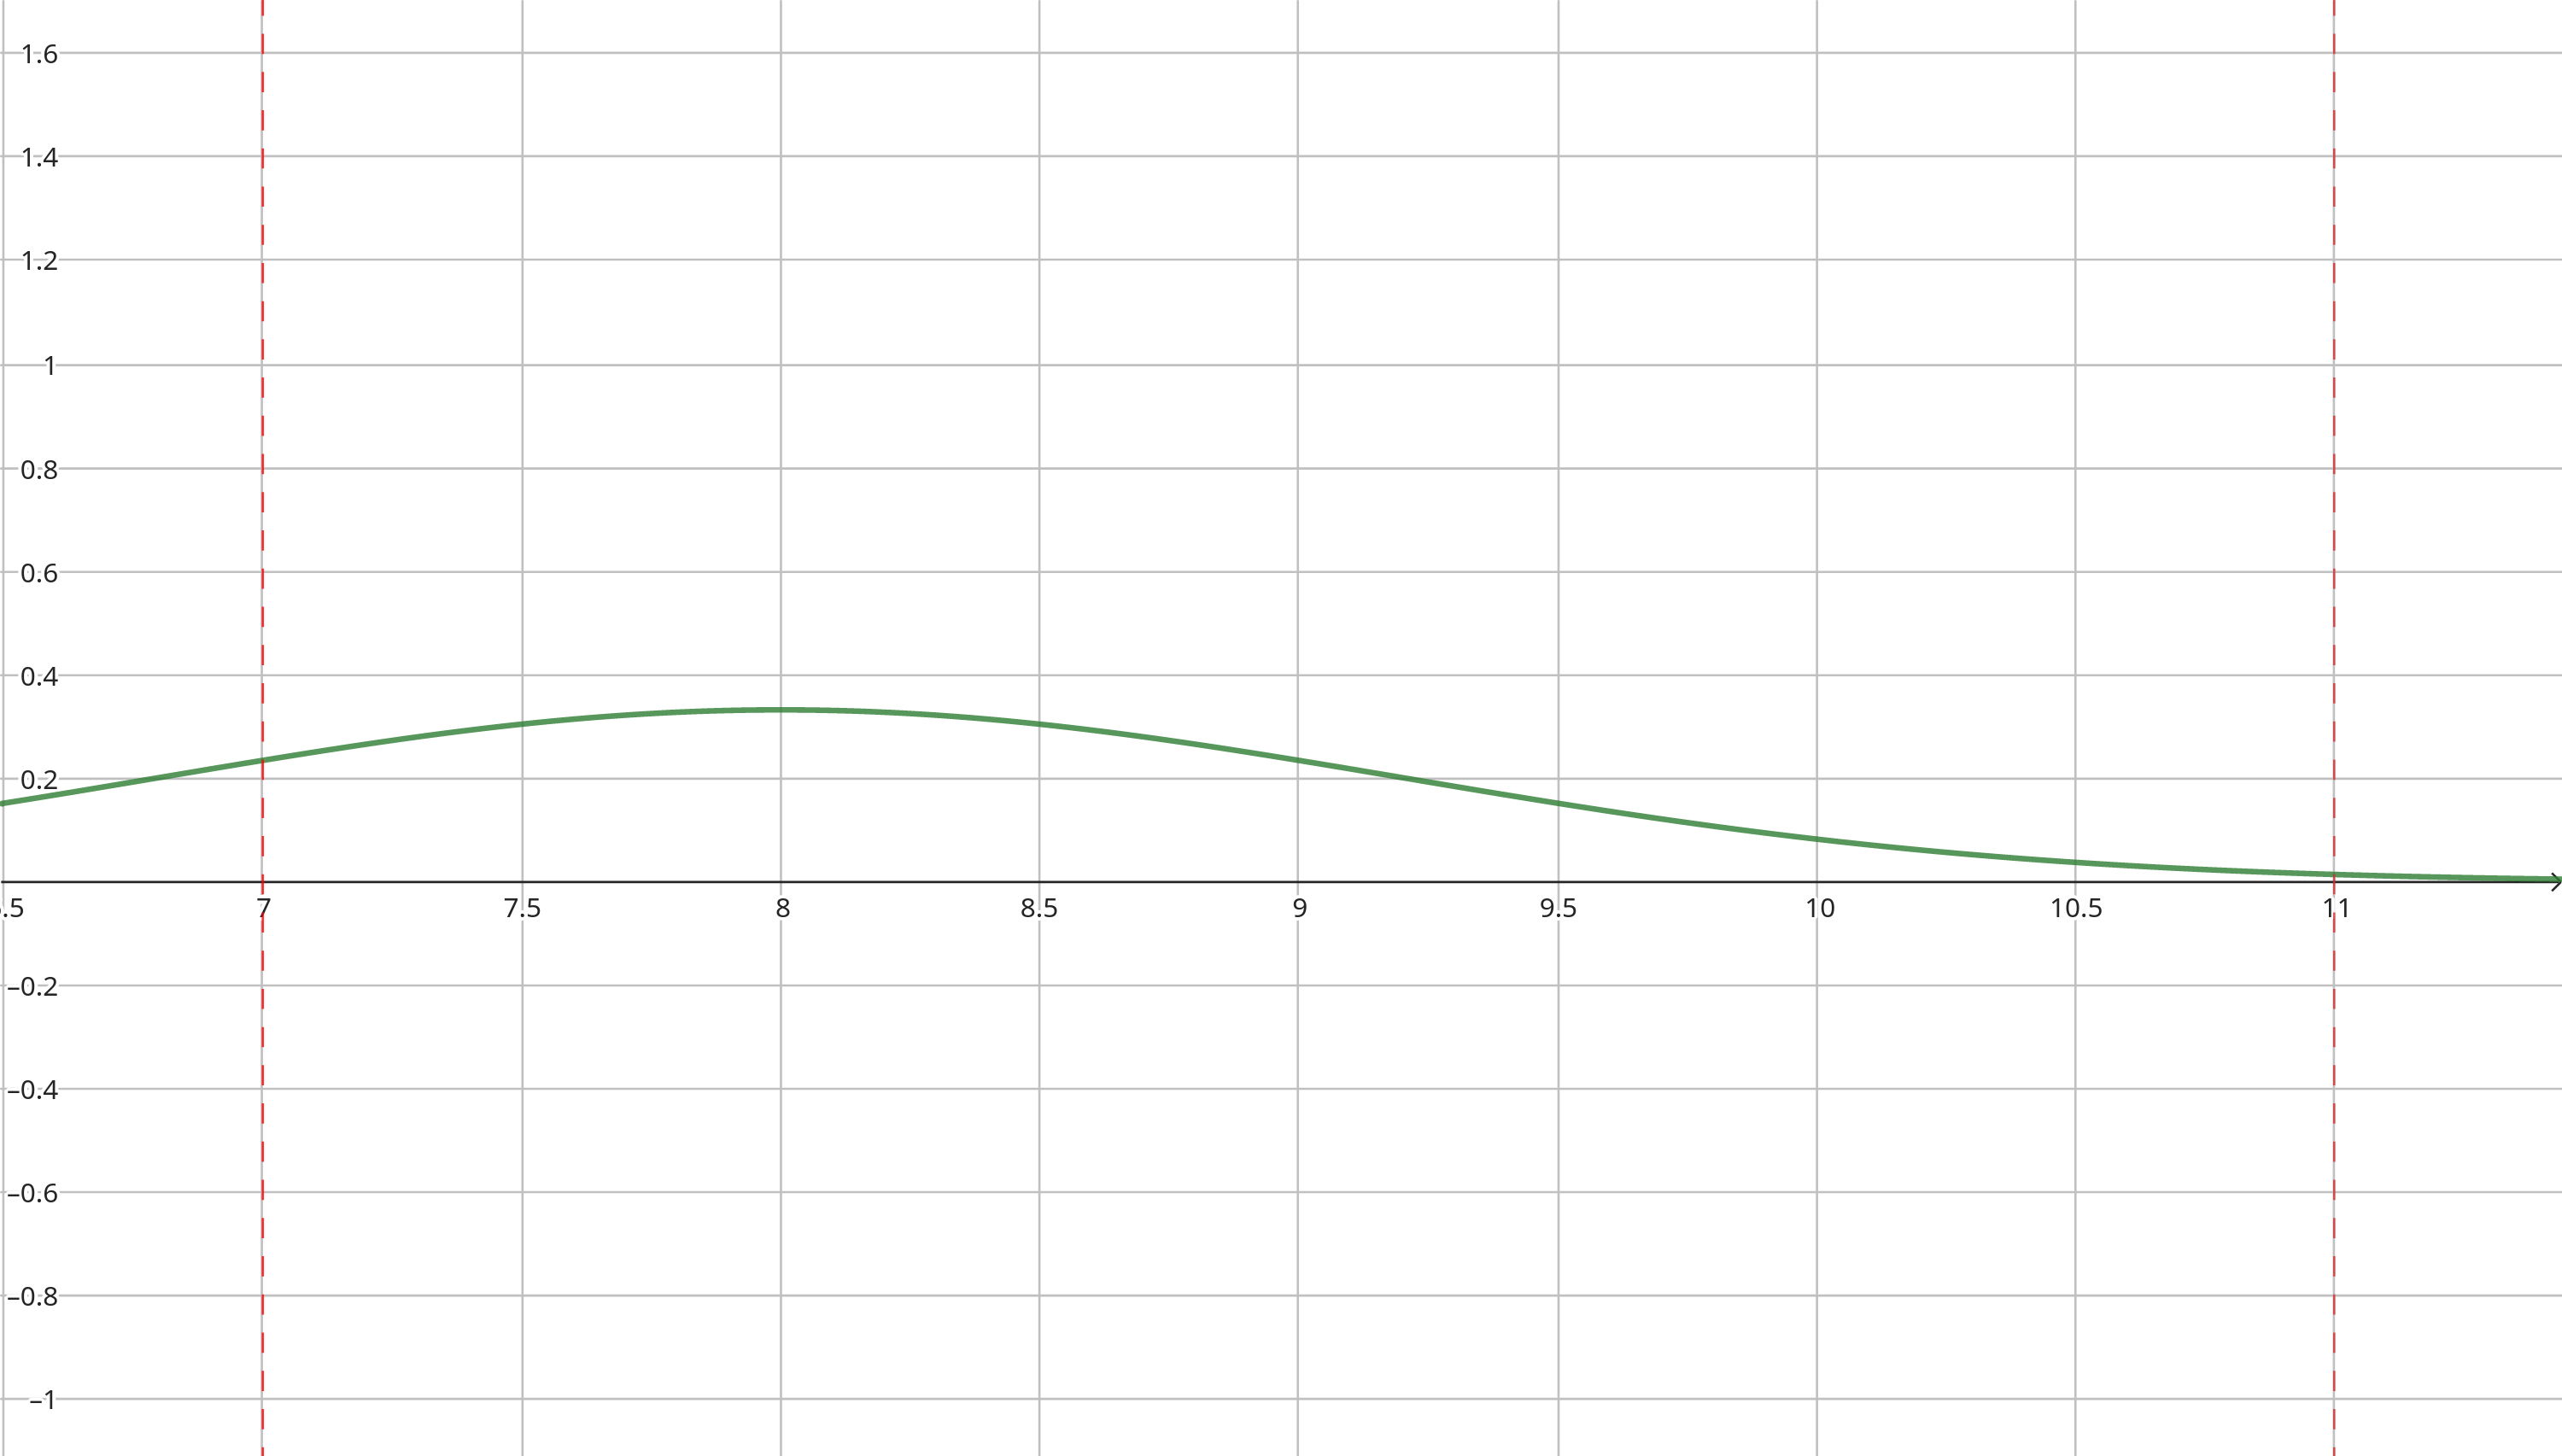
\includegraphics[width=\textwidth]{7-11-gaussian}
\centering \textit{Fascia oraria: 07:00 $\rightarrow$ 11:00}
\[ \mu = 8;\ \sigma = 1.2 \]
\end{figure}
\begin{figure}
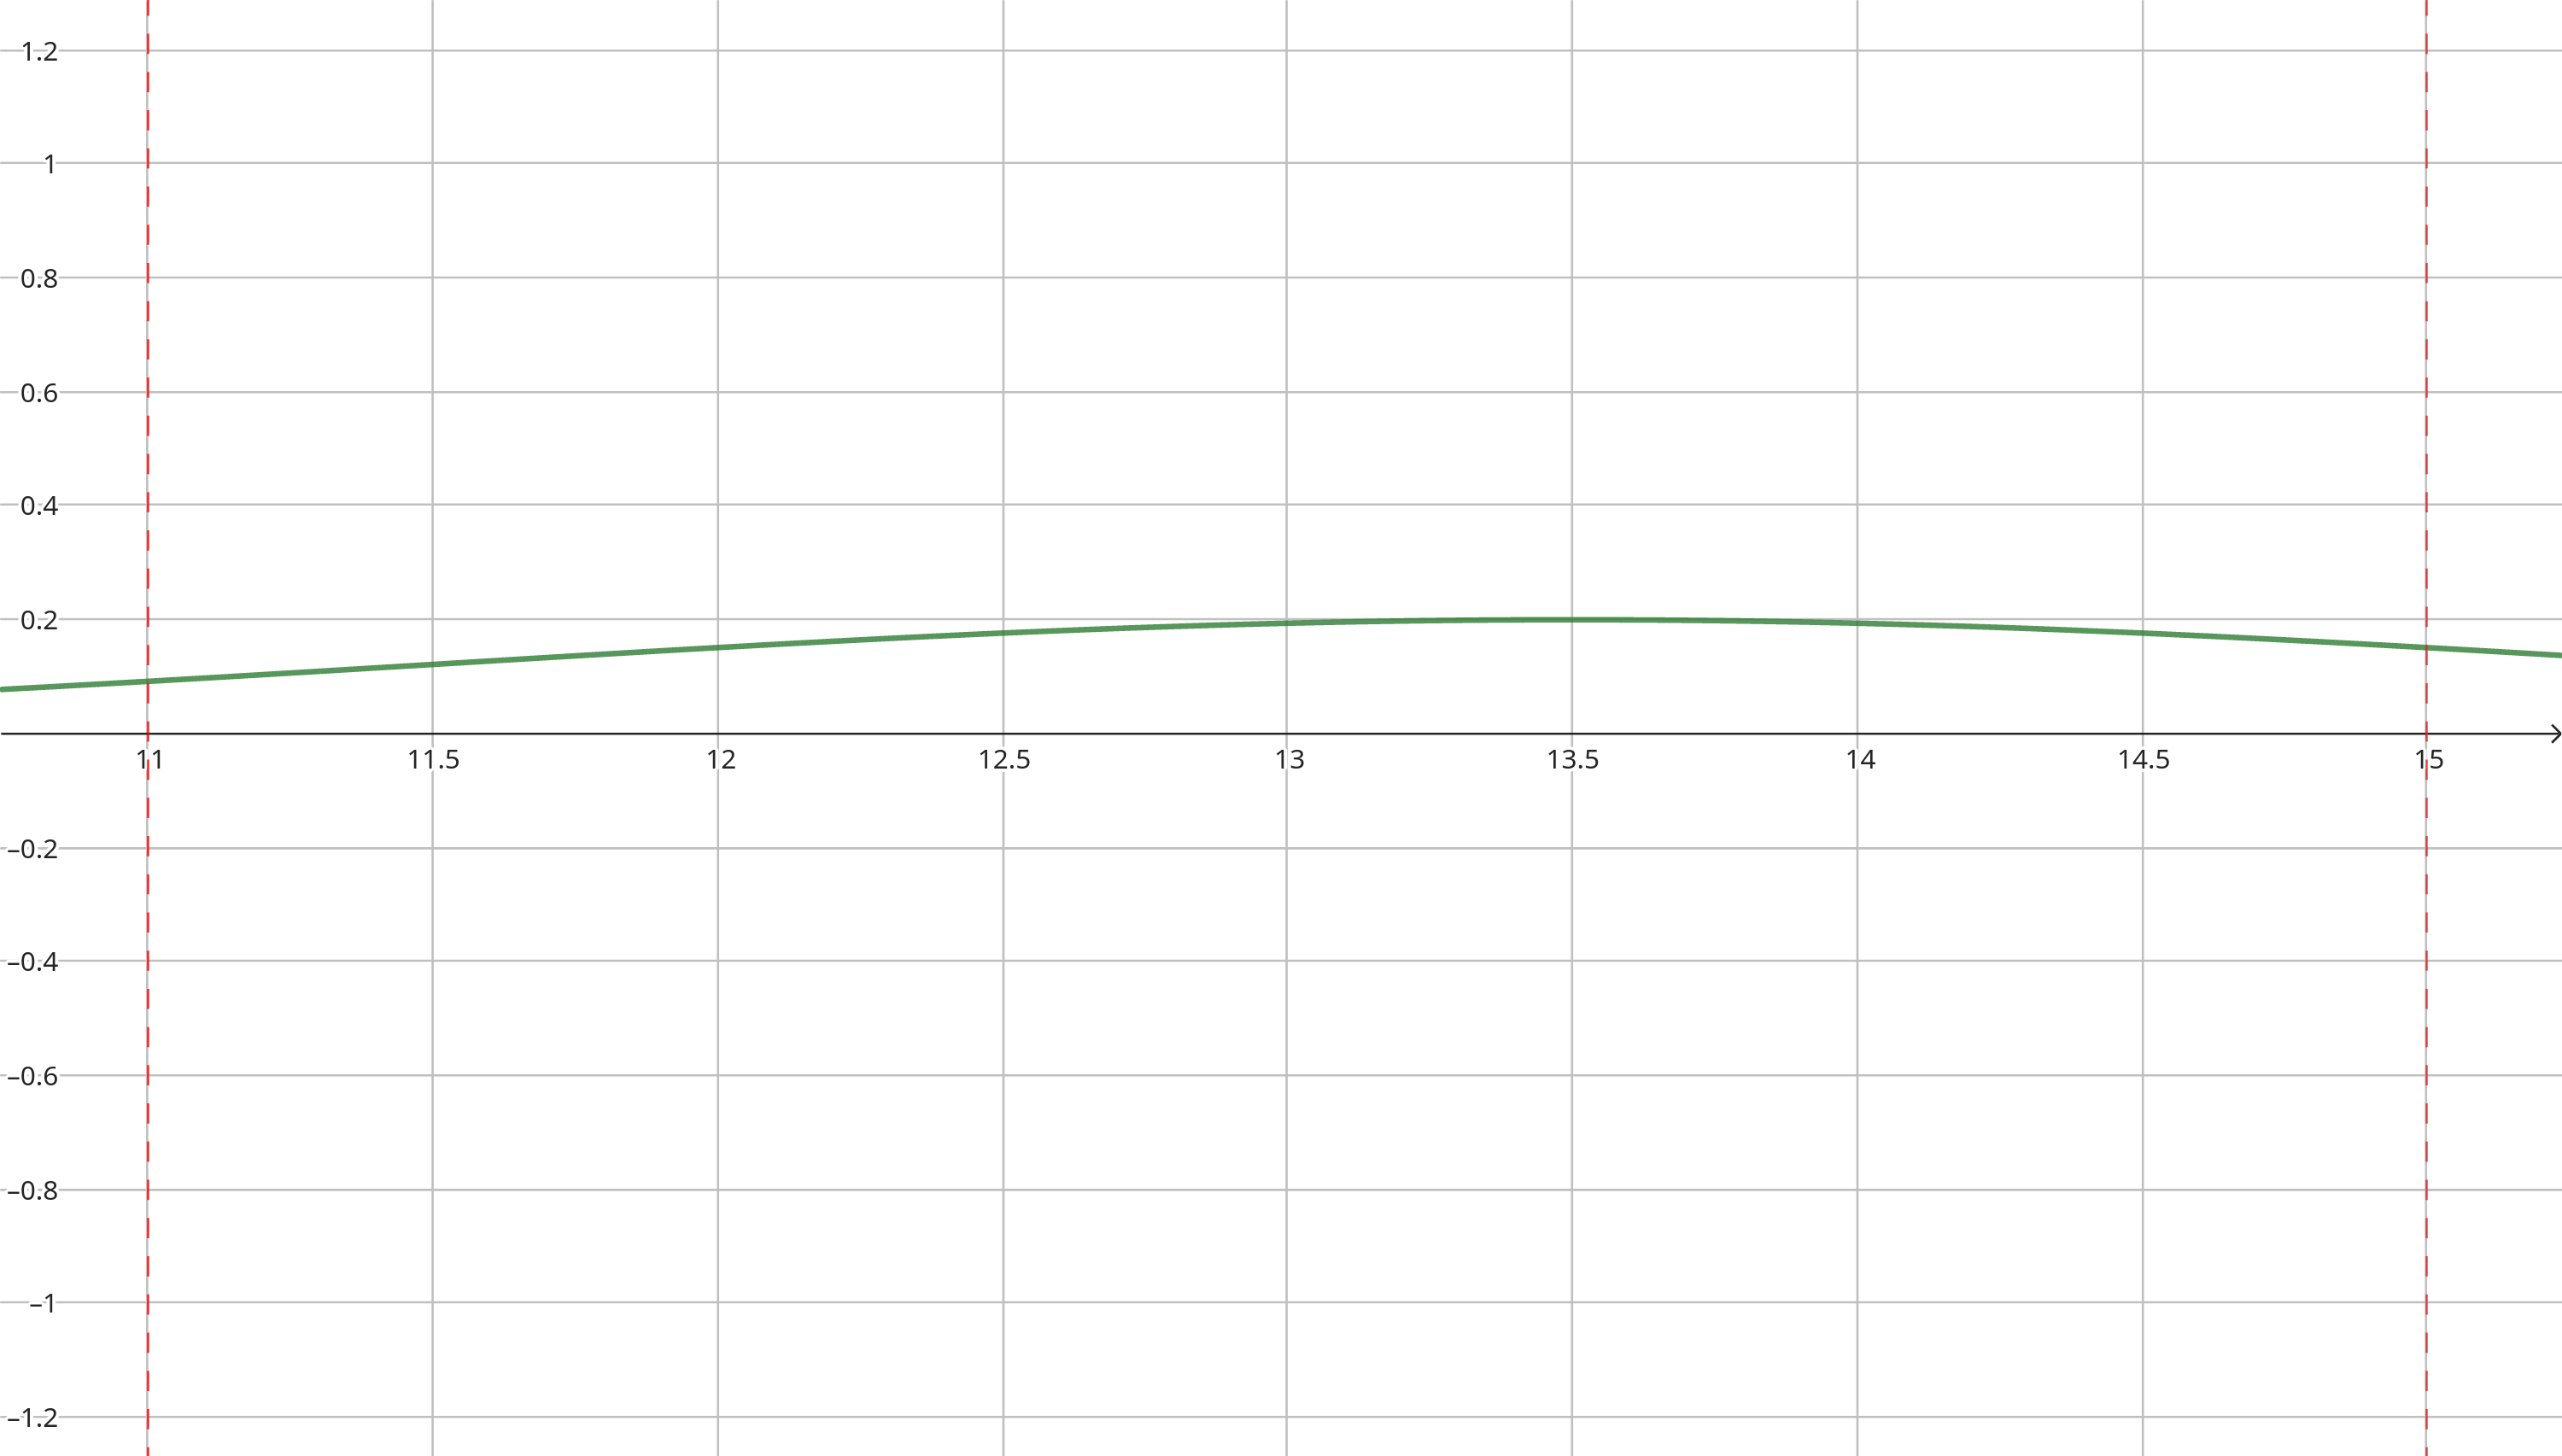
\includegraphics[width=\textwidth]{11-15-gaussian}
\centering \textit{Fascia oraria: 11:00 $\rightarrow$ 15:00}
\[ \mu = 13.5;\ \sigma = 2 \]
\end{figure}
\begin{figure}
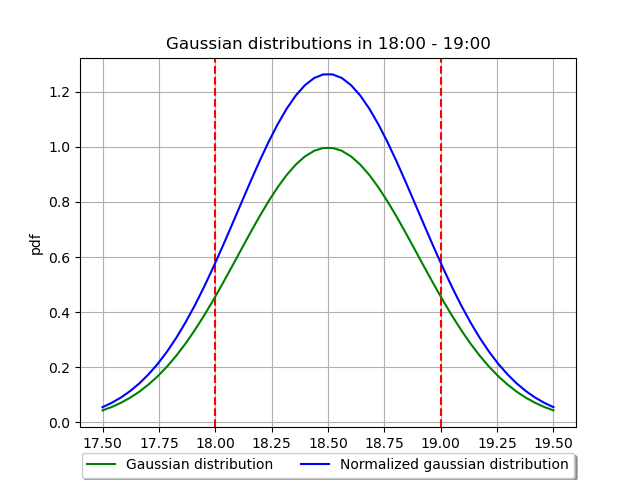
\includegraphics[width=\textwidth]{18-19-gaussian}
\centering \textit{Fascia oraria: 18:00 $\rightarrow$ 19:00}
\[ \mu = 18.5;\ \sigma = 0.4 \]
\end{figure}
\begin{figure}
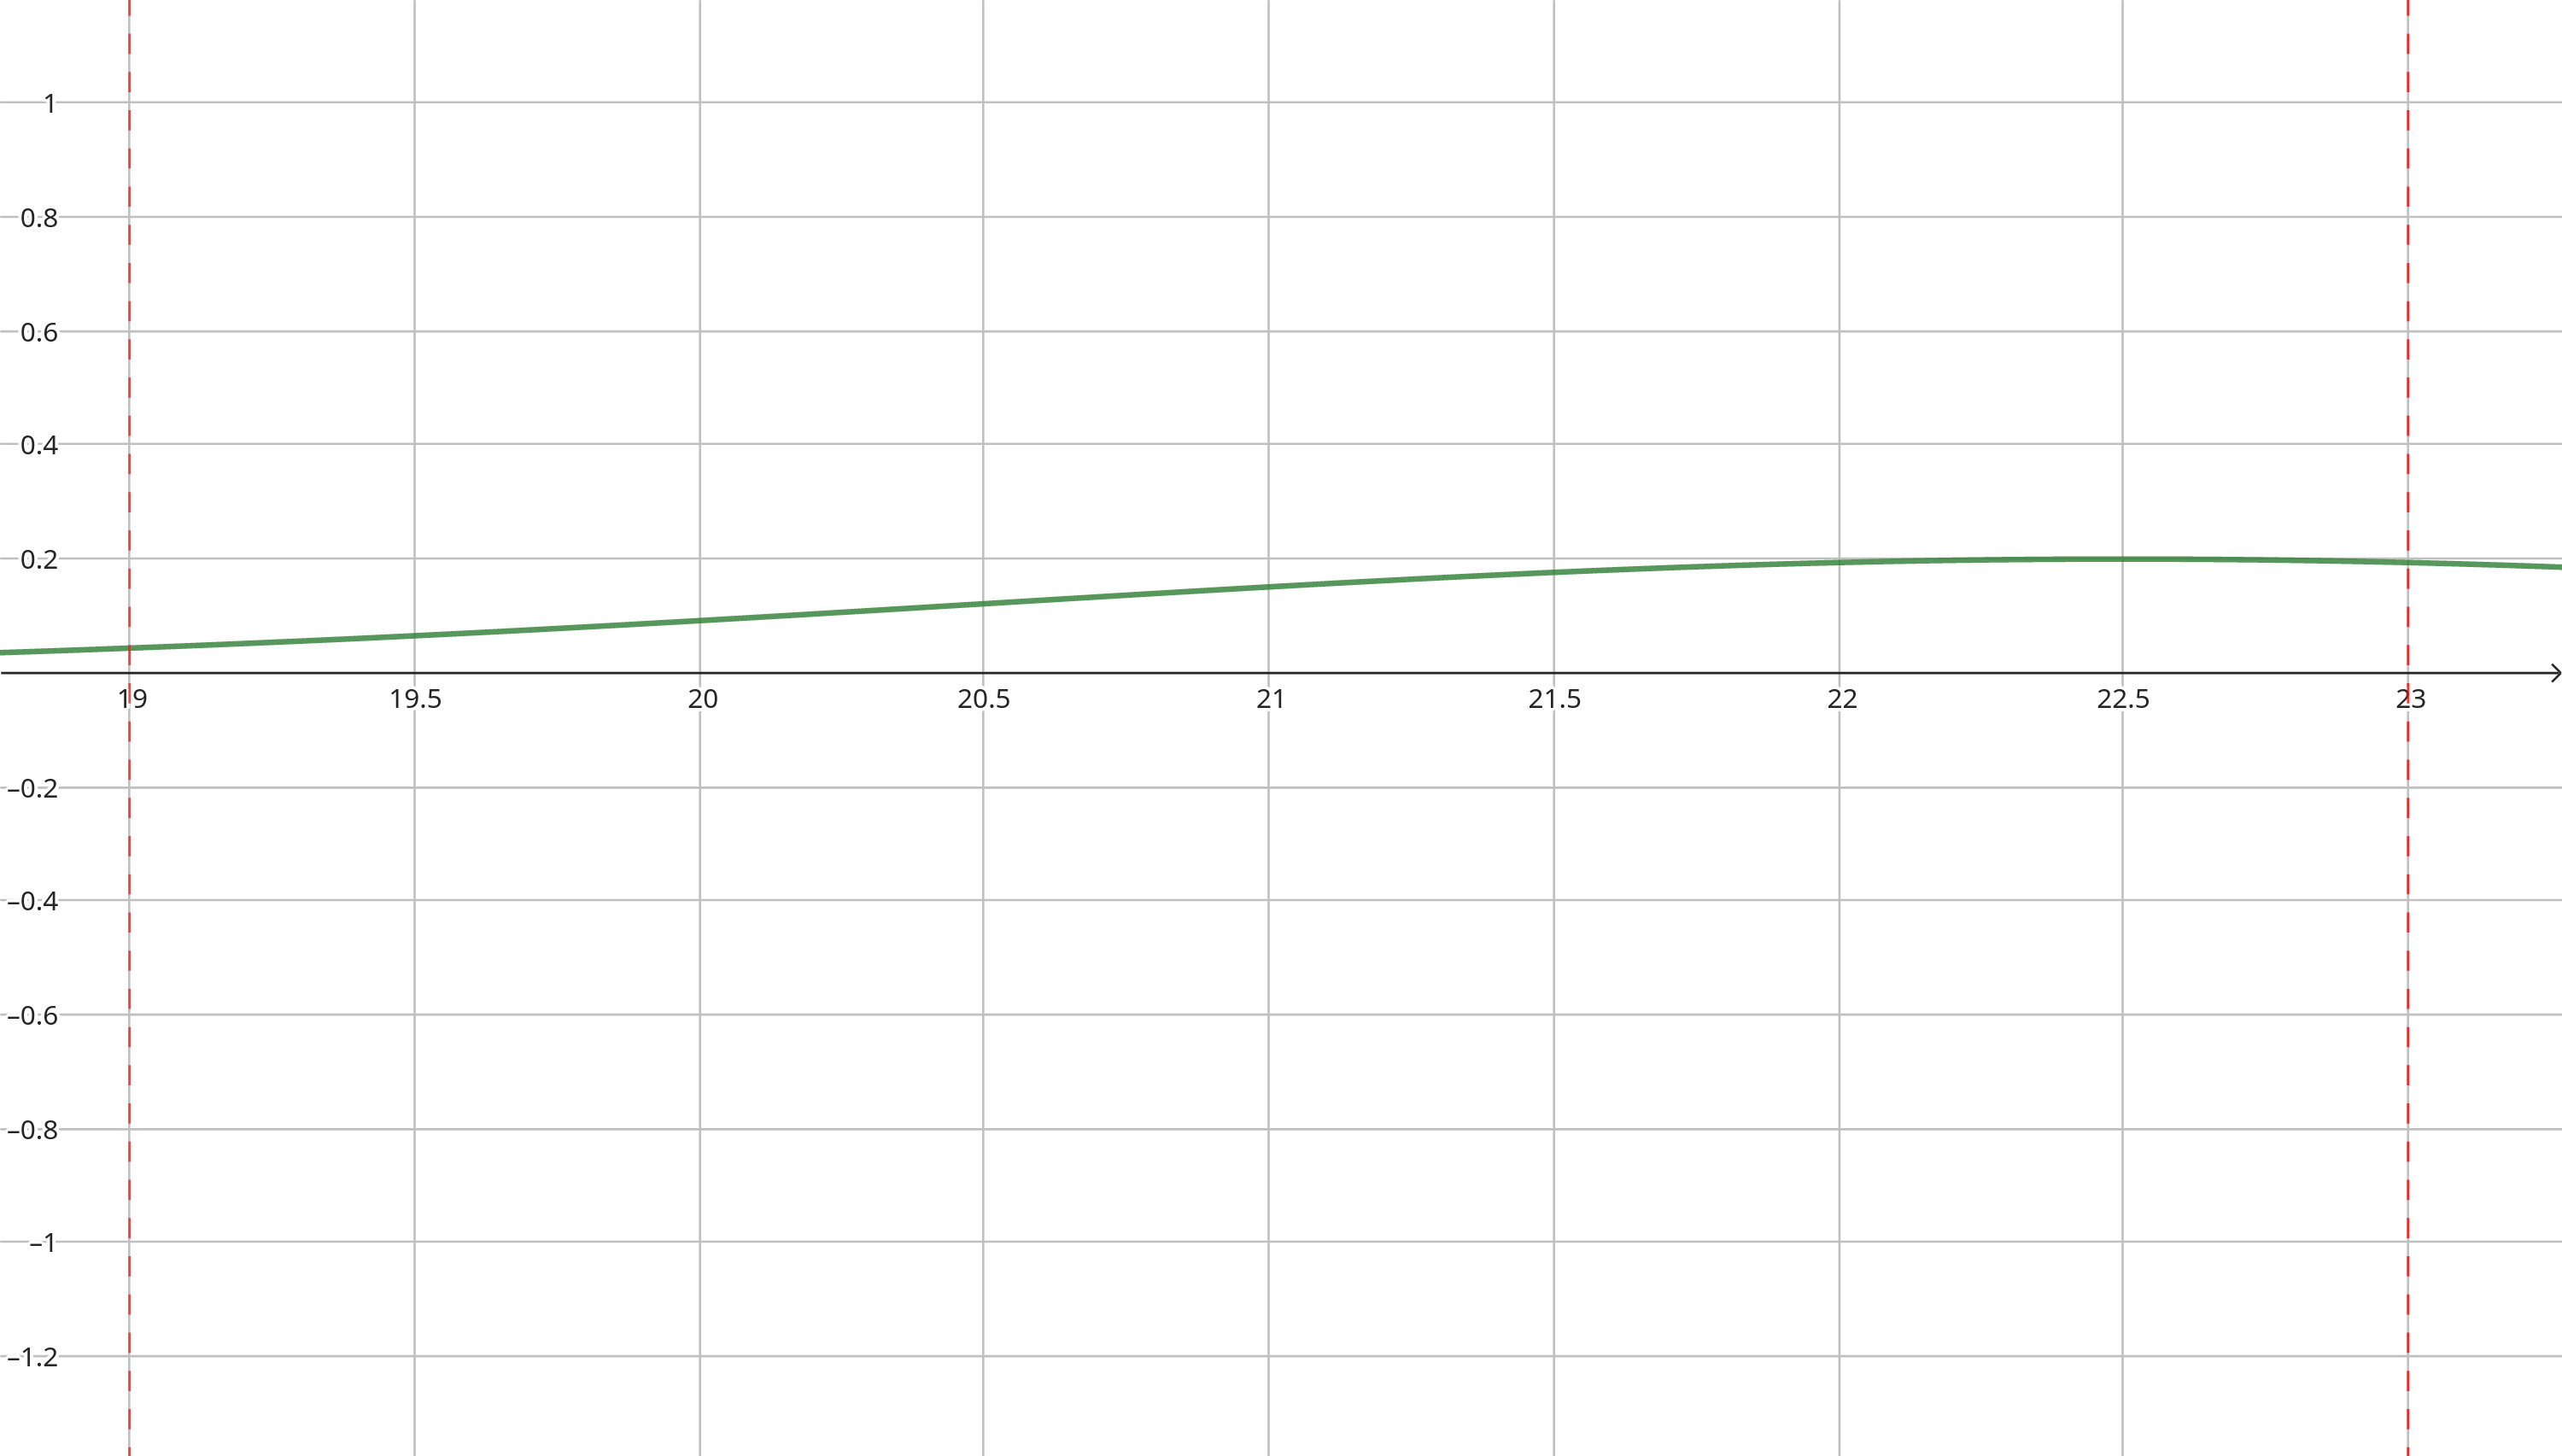
\includegraphics[width=\textwidth]{19-23-gaussian}
\centering \textit{Fascia oraria: 19:00 $\rightarrow$ 23:00}
\[ \mu = 22.5;\ \sigma = 2 \]
\end{figure}

\begin{figure}
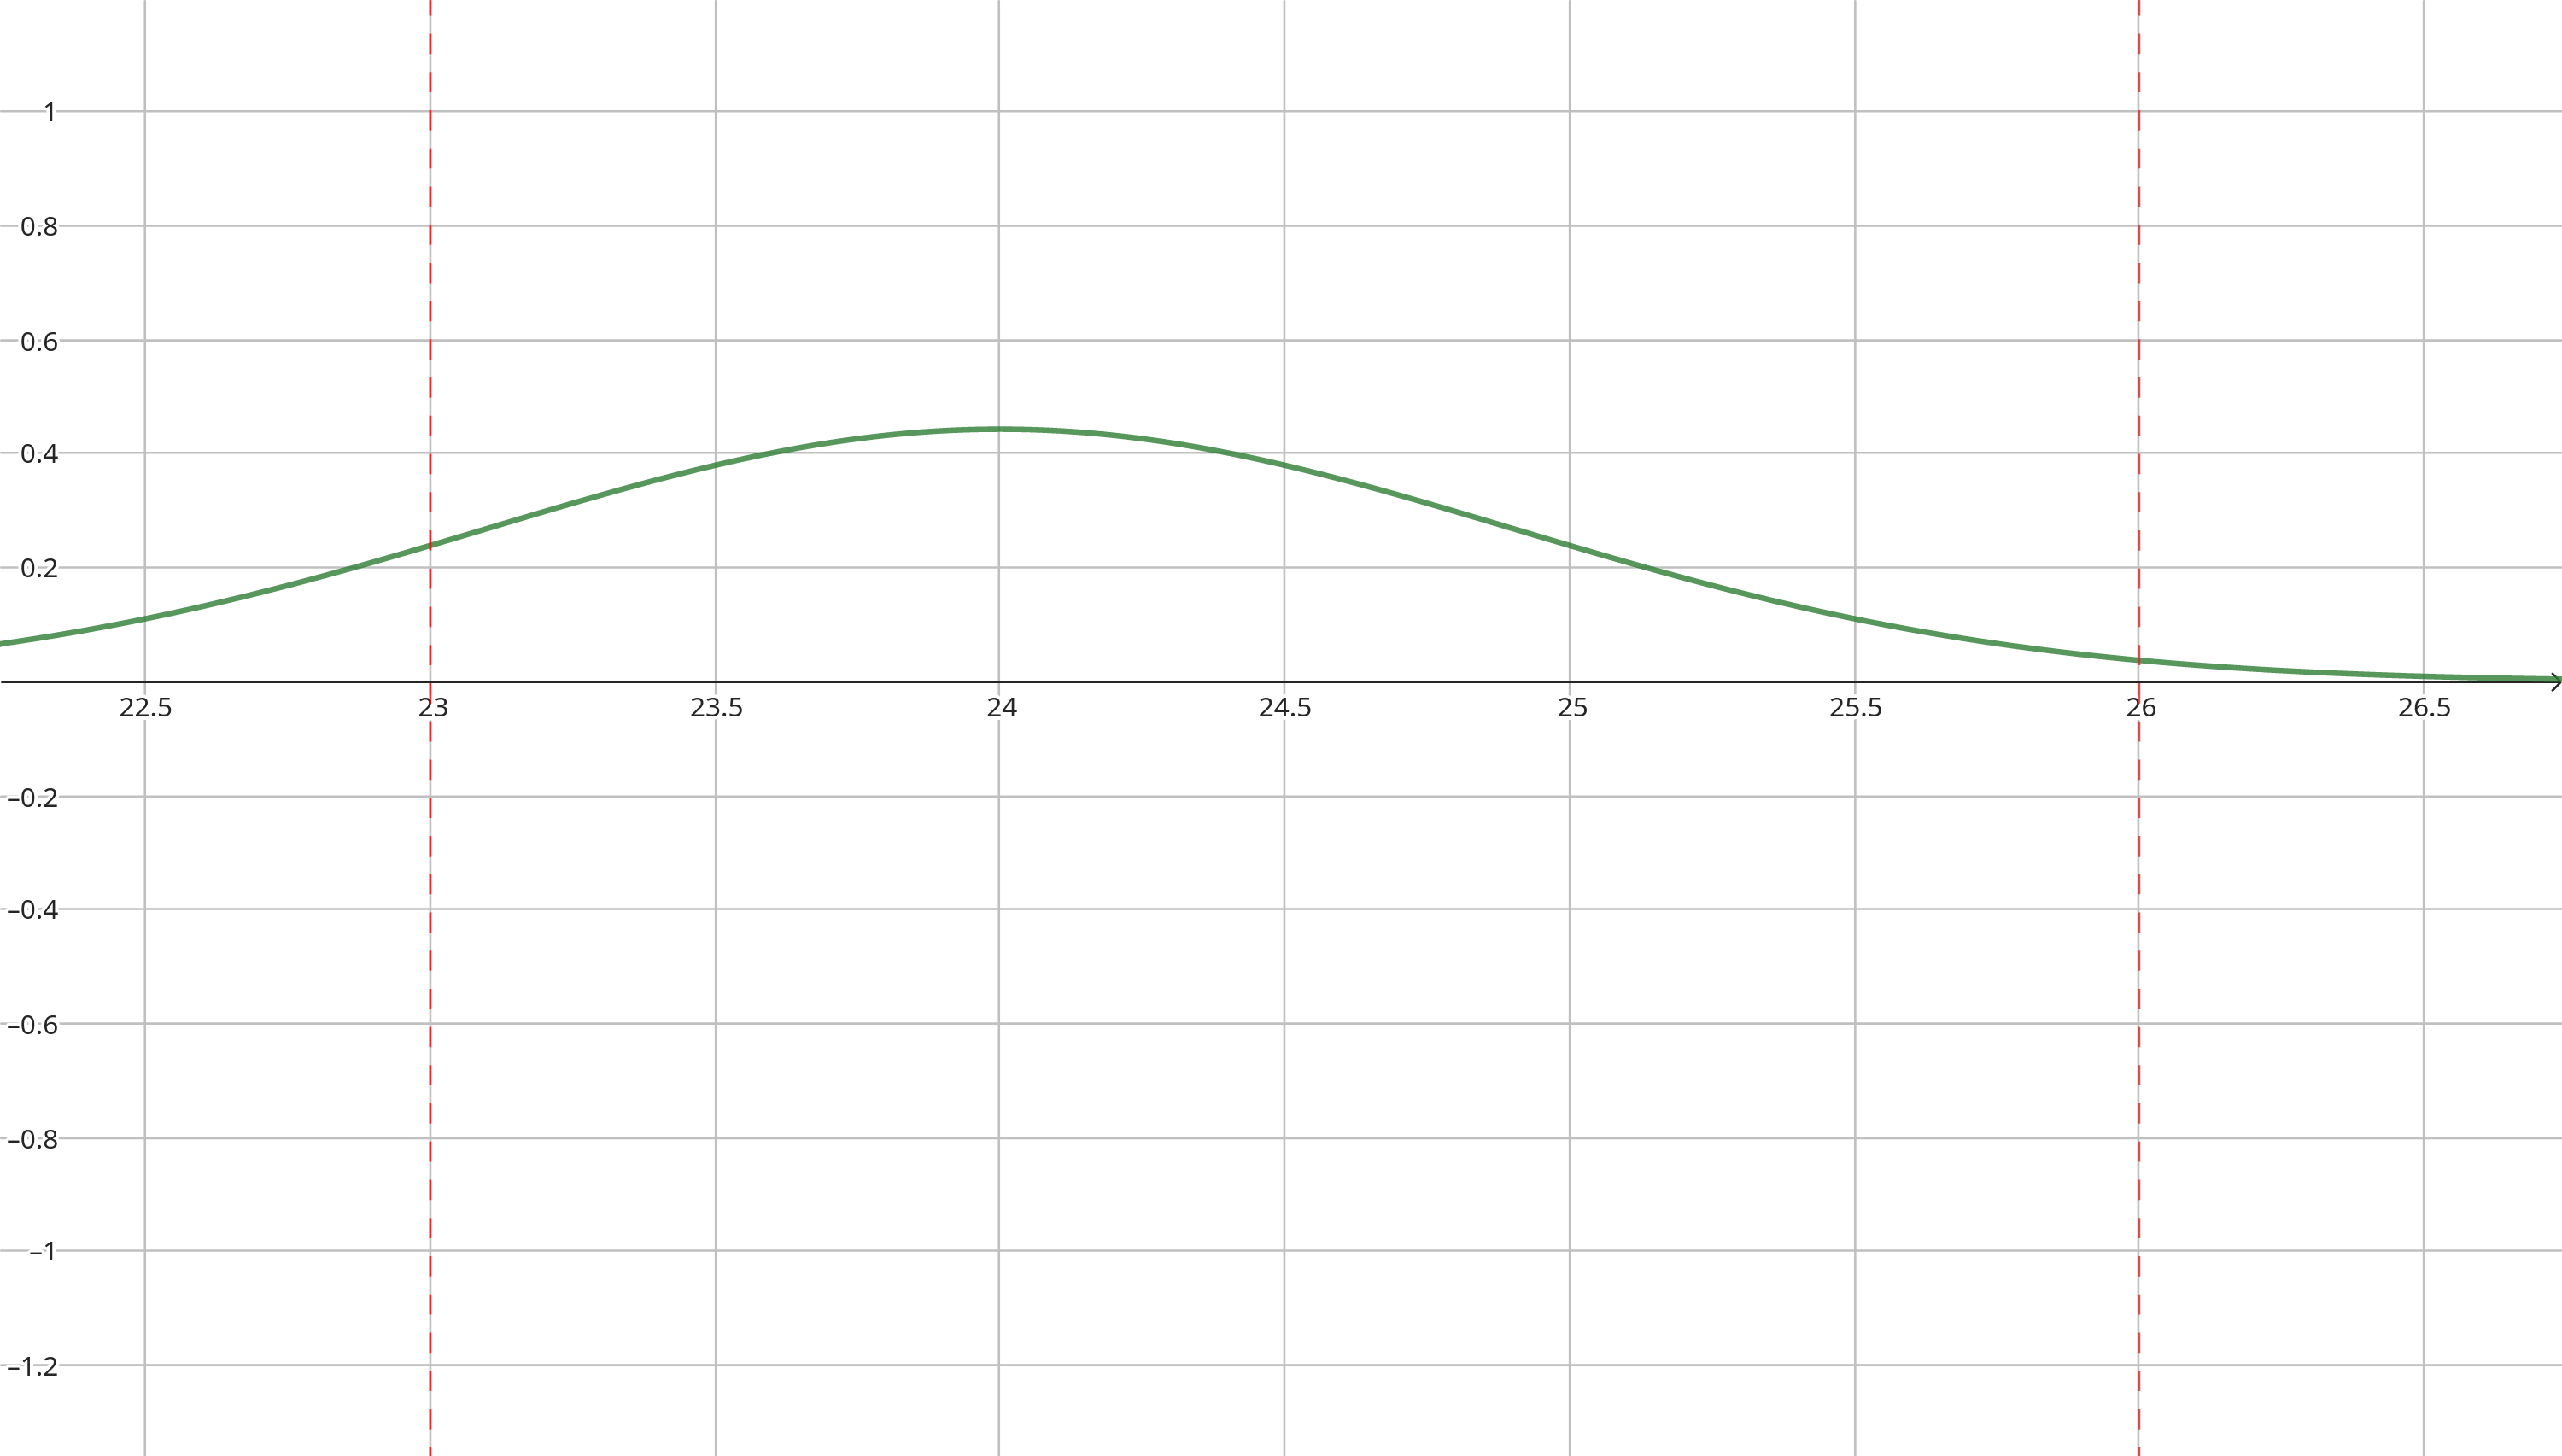
\includegraphics[width=\textwidth]{23-02-gaussian}
\centering \textit{Fascia oraria: 23:00 $\rightarrow$ 02:00}
\[ \mu = 24;\ \sigma = 0.9 \]
\end{figure}

\end{document}
